\begin{figure}[htbp]
	\centering
	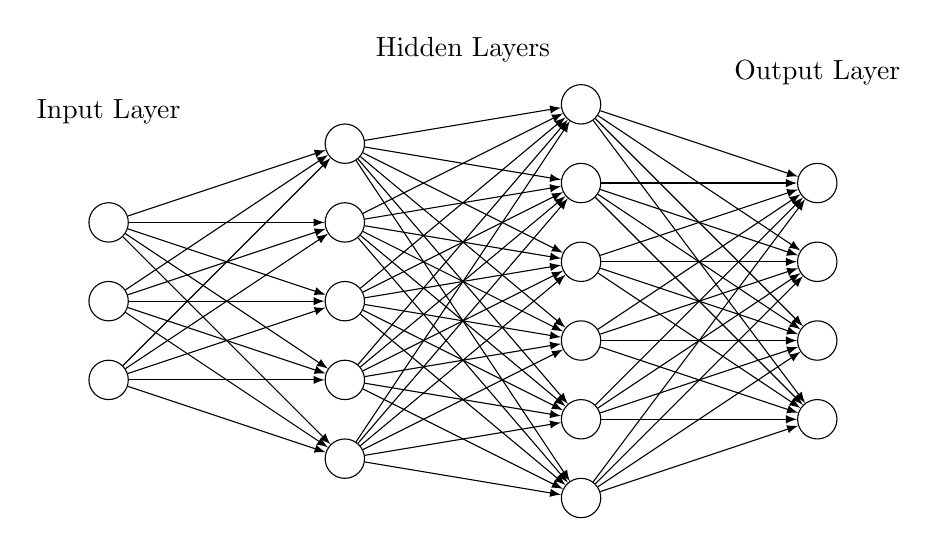
\begin{tikzpicture}[scale=1,every path/.style={>=latex}]
		%draw text nodes
		\node at (0,4.4) {Input Layer};
		\node at (9,4.9) {Output Layer};
		\node at (4.5,5.2) {Hidden Layers};
		% draw first layer
		\foreach \x in {1,...,3}
		{
			\node (n0\x) at (0, \x) [circle,draw,minimum size=0.5cm] {};
		}
		%draw second layer
		\foreach \x in {0,...,4}
     	{
     		\node (n3\x) at (3, \x) [circle,draw,minimum size=0.5cm] {};
     		% draw connections from layer one to layer two
     		\foreach \n in {1,...,3}
     		{
     			\draw[->] (n0\n) to (n3\x);
     		}
     	}
     	%draw third layer
		\foreach \x in {0,...,5}
     	{
     		\node (n6\x) at (6, \x - 0.5) [circle,draw,minimum size=0.5cm] {};
     		% draw connections from layer two to layer three
     		\foreach \n in {0,...,4}
     		{
     			\draw[->] (n3\n) to (n6\x);
     		}
     	}
     	%draw fourth layer
     	\foreach \x in {1,...,4}
     	{
     		\node (n9\x) at (9, \x - 0.5)  [circle,draw,minimum size=0.5cm] {};
     		% draw connections from layer three to layer four
     		\foreach \n in {0,...,5}
     		{
     			\draw[->] (n6\n) to (n9\x);
     		}
     	}
	\end{tikzpicture}
	\caption{Fully connected feed-forward neural network with two hidden layers}
	\label{fig:ffnn}
\end{figure}
